\documentclass[a4paper]{article}
\usepackage[breaklinks]{hyperref} %Great Command
\usepackage{refstyle}
\usepackage{float}
\usepackage{multirow}
\usepackage{graphicx}
\graphicspath{{./Pictures/}}
\usepackage{caption}
\usepackage{fancyhdr} % for a fancy header

\newcommand{\faculty}{Department of Mechanical Engineering, Ktirio M\\
National Technical University of Athens\\
Heroon Polytechniou 9\\
15780 Zografou, GREECE\\}

\renewcommand{\headrulewidth}{0.4pt}
\renewcommand{\footrulewidth}{0.4pt}
\title{Digital Pump XP3000 User Interface}
\author{Nikolaos L. Koukis}

\begin{document}

\maketitle
\tableofcontents
\listoffigures
\pagebreak
\section{Getting Started}

\subsection{About the software}
For the development of the GUI, the PySide\footnote{\url{http://qt-project.org/wiki/pyside}}
framework was used. For the editing part Vim\footnote{\url{http://www.vim.org}} was used.
Please refer to section~\ref{sec:license} for license information
regarding the source code and the redistribution policy.

\section{Hardware Setup}
\subsection{Equipment Used}
For the hardware communication to be achieved the following equipment is suggested:
\begin{itemize}
    \item USB\verb|->|Serial (RS-232) adapter
    \item RS-232\verb|->|RS-485 converter
    \item Power cables (Power + GND)
    \item Jumper wires (at least 2 Female to Male)
    \item Breadboard (optional)
\end{itemize}
\subsection{Connecting the XP3000}
The serial communication with the pump was implemented using the RS-485 serial
protocol. Here is a sample configuration that was used:

\begin{figure}[H]
    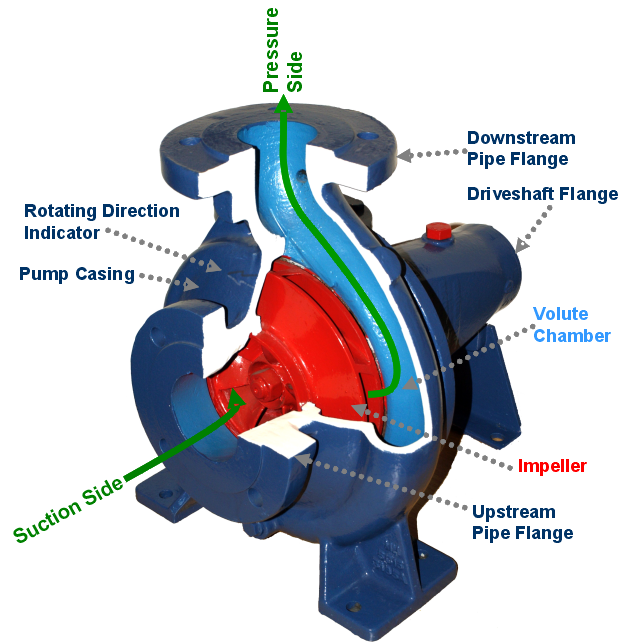
\includegraphics[width=0.8\textwidth]{RS-485-conf}
    \caption{RS-485 - Typical configuration}
    \label{fig:RS-485}
\end{figure}
The needed steps to achive a similar connection would be the following:
\begin{itemize}
    \item First you have to supply the pump with the necessary power. As described in the 
    manual the XP3000 requires a \emph{24VDC power supply} with a current rating of \emph{at least 1.5A}.
    As seen in \figref{RS-485}, during the development part, the power was supplied indirectly to the pump
    first by running the supply cables into a breadboard and then using extra jumpers to 
    connect to pump pins \#1 (power) and \#9(GND)
    \item For the serial communication, you need to connect the RS-485A, RS-485B signals from the pump PCB
    into the RS-485+, RS-485- of the data terminal (PC) used for the communication.
    Take exta notice when it comes to connecting the jumpers from the serial adapter
    to the pump PCB corresponding pins\\
\end{itemize}

To sum it up, here is the typical RS-485 pinout for the pump, as it is described above
\footnote{for a detailed breakdown of the pin positions and roles, consult the pump manual}:\\
    \begin{tabular}{ |l|l|l| }
        \hline
        \multicolumn{3}{ |c| }{RS-485 pin configuration} \\
        \hline
        Role & Pin No.~ & Signal to connect\\ \hline
        \multirow{2}{*}{Power} & \#1 [Power] & 24VDC \\
        & \#9 [GND] & Ground(of the power supply)\\ \hline
        \multirow{2}{*}{Protocol Signals} & \#11 [RS485B] & R-S485+\\
        & \#12 [RS-485B] & RS-485-\\ \hline
        \hline
    \end{tabular}

\section{Software Setup}
\subsection{Getting the Software}
There are two ways of acquiring and running the programme,
You can either download directly the executable, extract and run the window\_controller.exe
, or you can download the source code and run it using any python distribution.

\begin{description}
    \item[Running the .exe file] \hfill\\
        This option is pretty straightforward. A zipped version of the executable 
        can be downloaded from: \url{a}.%TODO
        After the download completes, extract it with the tool of your choice and 
        run it
    \item[Running from source] \hfill\\
        In order to directly run the python source you need to have the following modules
        in your \textit{PYTHONPATH}:
        \begin{itemize}
            \item PySide (tested on PySide 1.2.2)
            \item serial
            \item signal
            \item Queue
            \item threading
        \end{itemize}
        For *nix users, downloading the needed modules 
        is pretty straightfoward (either from source or using pip). 
        For windows users, getting a full python distribution is recommended (i.e \href{https://www.enthought.com/}{Enthought-Canopy}, \href{http://www.continuum.io/}{Anaconda})
        which are shipped with most of the above modules already installed and ready
\end{description}

\subsection{User Interface}
The first thing you have to do when you try to connect to the pump is to discover the computer port it is running on
For \emph{Windows users} this can be done in the following way:
\begin{enumerate}
    \item Start Menu, right click on the `My Computer' button and select `Manage'
    \item Click on the `Device Manager' tab
    \item Click on the `Ports (COM \& LPT)' tab and then select the port your adapter is on
\end{enumerate}

For *nix users (Linux, MacOs etc.) this can be done in the following way:
\begin{enumerate}
    \item Open the terminal application
    \item Issue the following commands:
        \begin{quote}
            cd /dev\\
            ls -lart \verb+|+grep tty\\
        \end{quote}
        This will give you a list of the available ports.
        Run the second command after ejecting and inserting again the serial adapter 
        so that you can discover the needed port
    \item Click on the `Ports (COM \& LPT)' tab and then select the port your adapter is on
\end{enumerate}
Make sure that \emph{you have selected the correct port}, otherwise the pump will not respond and will
not raise any error Message

After running the software you will be prompted with the \emph{New Device Dialog}.
Select the port on which the pump is connected.
%TODO insert picture
You are now in the \emph{Main Window Screen}. From here you can command a volume delivery,
change the speed of the plunger, or issue a quick command to the pump 
\textit{push al the fluid, full the syringe etc.}
You can also select the editor's tab in order to issue a series of commands to the pump 
and either run it or save it for later use.
A typical view of the main window is the following, running on a MacOs 10.9 environment:
%TODO insert picture
From the main window screen you can navigate to a series of other dialog windows

\section{Contact Information}
\noindent{For information, bug reports, or just to drop a comment about the software,
contact using one of the methods below:}

\begin{tabular}{ll}
    \textbf{by email:} & nickkouk@gmail.com\\
    \textbf{by phone:} & +30 210 7721516\\
\end{tabular}

\vspace{2 mm}
\noindent{\textbf{Mailing Address:}\\}
\faculty

\section{Appendix A: Software license}
\label{sec:license}
The Software is licensed under the LGPL v2.1\footnote{\url{http://www.gnu.org/licenses/old-licenses/lgpl-2.1.html}}.
The source code as well as the documentation code -- written in Latex -- is 
freely available for download and modification from the following github page:
\url{https://github.com/bergercookie}.
Everyone interested, is encouraged to contribute in the developement of the program
either by suggesting changes to the UI or by working on the open issues\footnote{This should be the link to that!}of the software
%TODO!! enter an open issues tracker in github

\section{Appendix B: Pump Commands}
The commands below consist the main way for communicating with the pump.
They can be given directly by the user from the Editor Tab.
The user can also issue common python commands according to his own
needs.

\subsection{\mbox{pump.send\_Command(self, command, bits\_on\_return = 0)}}
\textbf{Arguements}
\begin{itemize}
    \item command \verb|->| python string
    \item bits\_on\_return \verb|->| integer [default value = 0]
\end{itemize}
\textbf{Description}\\
Sending Commands to the pump.
Consult the manual for a detailed list of the pump commands for the RS-485 Protocol. 
Using this method you must have already defined the pump address to send to (Via
the main window or the Editor tab) and you should issue neither 
the Run character [R] nor the terminating character [$\backslash$r]\\
\textbf{Examples}\\
pump.send\_Command(`A3000', 10) \verb|->| move the plunger to abs position 3000, read back 10 bytes\\
pump.send\_Command(`T') \verb|->| Terminate Plunger move in progress

\subsection{\mbox{pump.connect\_new(self, port\_name)}}
\textbf{Description}\\
Connect to the given serial port address.
Make sure that the given port address isn't already in use\\
\textbf{Examples}\\
pump.connect\_new(`/dev/tty.-SerialPort1-1') \verb|->| Configuring connection on Mac

\subsection{\mbox{pump.initialize\_pump(self, output = `right')}}
\textbf{Description}\\
Initialize the default output valve. The default output value,
unless indicated differently is the right valve
\textbf{Examples}\\
pump.initialize\_pump() \verb|->| Initializing the pump with default output valve (right)\\
pump.initialize\_pump(output = `left') \verb|->| Initializing the pump with output valve set to left\\

\subsection{\mbox{pump.valve\_command(self, position)}}
\textbf{Arguements}
\begin{itemize}
    \item Input\_Valve: `I'
    \item Output\_Valve: `O'
    \item Bypass\_Valve: `B'
\end{itemize}
\textbf{Description}\\
Set the valve to certain position\\
\textbf{Examples}\\
pump.valve\_command(`B') \verb|->| Set the valve to Bypass position

\subsection{\mbox{pump.property\_set(self, a\_property, value)}}
\textbf{Arguements}\\
%TODO insert as items
\begin{tabular}{ll}
    Property\_str,& [Command,[Setting\_Limits]]\\
    `speed':& [`S', [1, 40]]\\
    `backlash':& [`K', [0, 31]]\\
    `slope':& [`L', [1, 20]]\\
    `start\_velocity':& [`v', [50, 1000]]\\
    `top\_velocity':& [`V', [5, 5800]]\\
    `cutoff\_velocity':& [`c', [50, 2700]]\\
    `cutoff\_velocity\_steps':& [`C', [0, 25]]\\
\end{tabular}

\noindent{\textbf{Description}\\}
The user can specifically set a property of the pump to a specific value\\
\textbf{Examples}\\
pump.property\_set(`speed', `10') \verb|->| Set the plunger speed to 10\\
pump.property\_set(`backlash', `15') \verb|->| set the backlash steps to 15

\subsection{pump.volume\_command(self, direction = `P', vol = `0' [in microlt],special=None)}
\textbf{Arguements}
\begin{itemize}
    \item special = `push\_all'
    \item special = `pull\_all'
\end{itemize}
\textbf{Description}\\
Volume Pushing / Drawing mechanism.
direction \verb|->| python\_string\\
vol \verb|->| python\_string [!]\\
The user can issue a special action as well.\\
\textbf{Examples}\\
pump.volume\_command(direction = `D', vol = `5') \verb|->| Dispense 5 microlitres\\
pump.volume\_command(special = `push\_all') \verb|->| Dispense fluid volume

\subsection{\mbox{pump.ser.write(string\_to\_pump)}}
\textbf{Description}\\
This command should be used when a direct serial command has to be sent to the pump.
User must issue the pump to which he is addressing to as well as the terminating character\\
\textbf{Syntax}\\
pump.ser.write(address + command + character\_to\_send + termination\_char)\\
\textbf{Examples}\\
pump.ser.write(`/2ZR\r') \verb|->| Initialize the pump with the address \textit{1}
\end{document}
